
\chapter{IEEE 802.15.4}

IEEE 802.15.4 is a standard specifying \textbf{physical} and \textbf{MAC} layers for low-rate wireless personal area networks (LR-WPANs).

It is infrastructure-less, short range and its Physical layer may coexist with IEEE 802.11 (Wi-Fi) and IEEE 802.15.1 (Bluetooth). 

\section*{Physical Layer}

The Physical layer may operate in three possible frequency bands:
\begin{itemize}
   \item 868.3 MHz (Europe)
   \item 902-928 MHz (Americas) (11 channels, 2 MHz each)
   \item 2.4 GHz (Worldwide) (16 channels, 5 MHz each)
\end{itemize}

The Physical Layer works well even in low \textit{Signal-to-noise ratio} (\texttt{SNR}) environments, and it is able to work with a very low power consumption.
In other words, it is less likely to misread a packet.
{\ns\note{For example, the ``shouting'' of the preamble in B-MAC increases the SNR.}}

\note{\begin{itemize}
   \item \textbf{Data Service}
   \begin{itemize}
      \item Transmission/Reception of PHY
      Protocol Data Unit (PPDU) through the physical
      medium.
   \end{itemize}
   
   \item \textbf{Management Service}
   \begin{itemize}
      \item Radio transceiver activation/deactivation (to
      implement policies of energy efficiency)
      \item Energy Detection - ED
      \item Link Quality Indicator - LQI
      \item Channel Selection
      \item Clear Channel Assessment - CCA
      \item PHY-PIB (PHY PAN Information Base) Configuration
   \end{itemize}
\end{itemize}}

\begin{figure}[htbp]
   \centering
   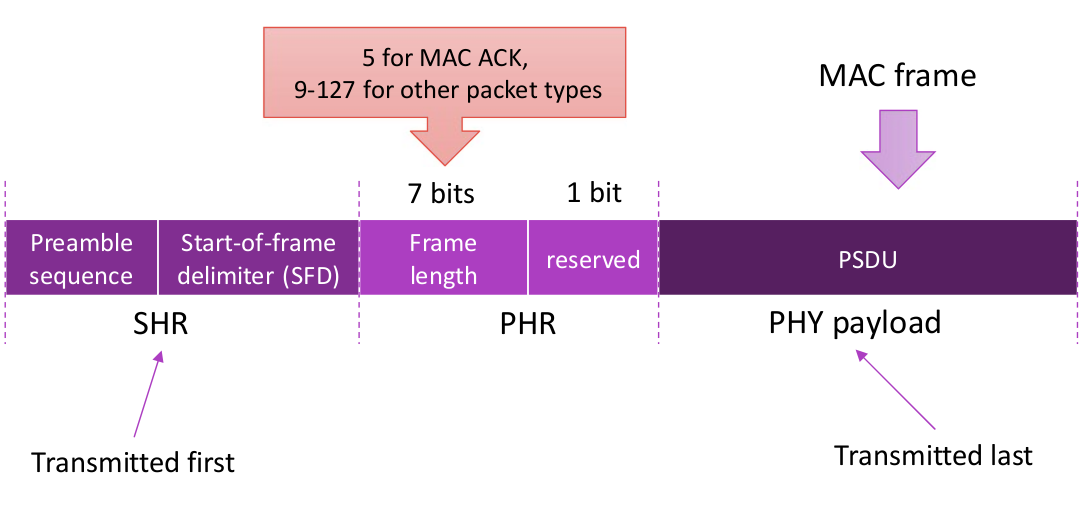
\includegraphics{images/802_physicalframe.png}
   \caption{Physical frame structure}
   \label{fig:802_physicalframe}

   \begin{itemize}
      \item \texttt{SHR} (Synchronization Header): synchronisation with the receiver
      \item \texttt{PHR} (PHY Header): information about the frame length
      \item \texttt{PHY} Payload: the MAC frame
   \end{itemize}
\end{figure}
   
\section*{MAC Layer}

MAC layer provides various services:
\begin{itemize}
   \item \textbf{Data services}
   \begin{itemize}
      \item transmission and reception of MAC frames (MPDU)
      across the physical layer.
   \end{itemize}
   \item \textbf{Management services}
   \begin{itemize}
      \item Synchronization of the communications
      \item Channel access
      \item Management of guaranteed time slots
      \item Association and disassociation of devices.
   \end{itemize}
   \item \textbf{Security services}
   \begin{itemize}
      \item Data encryption
      \item Access control
      \item Frame integrity
      \item Sequential freshness
   \end{itemize}
\end{itemize}

This layer defined two types of devices:
\begin{itemize}
   \item \textbf{Full-function device} (FFD): can act as a coordinator;
   \item \textbf{Reduced-function device} (RFD): cannot act as a coordinator.
\end{itemize}


At the MAC layer there may be different network topologies:
\begin{itemize}
   \item \textbf{Star}: a central FFD PAN coordinator communicates with all the other nodes, which may be either FFDs or RFDs.
   \begin{figure}[htbp]
      \centering
      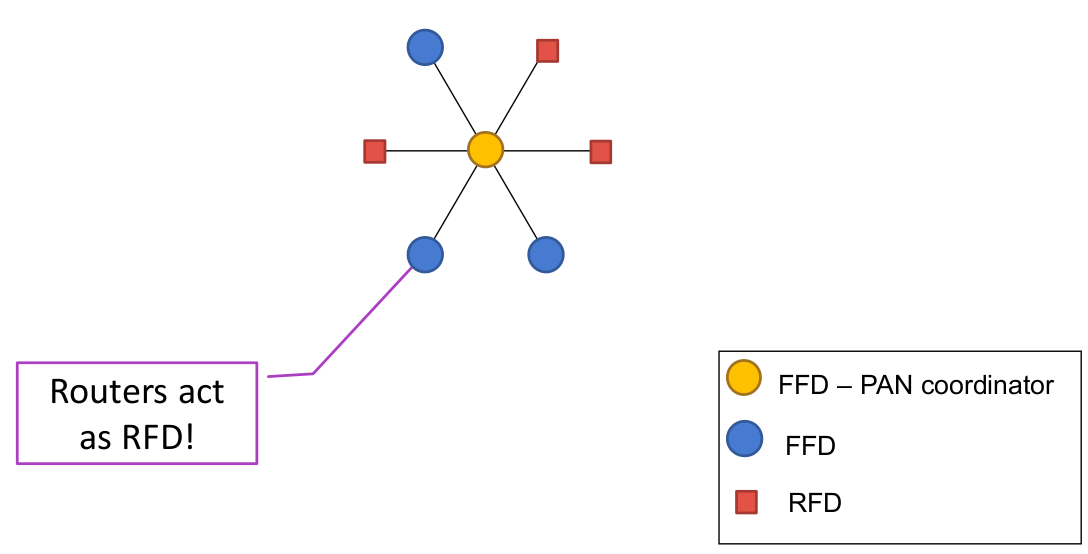
\includegraphics{images/802_star.png}
      \label{fig:802_star}
   \end{figure}
   \item \textbf{Peer-to-peer}: again there is a PAN coordinator, FFDs are routers and RFDs are end devices.
   \begin{figure}[htbp]
      \centering
      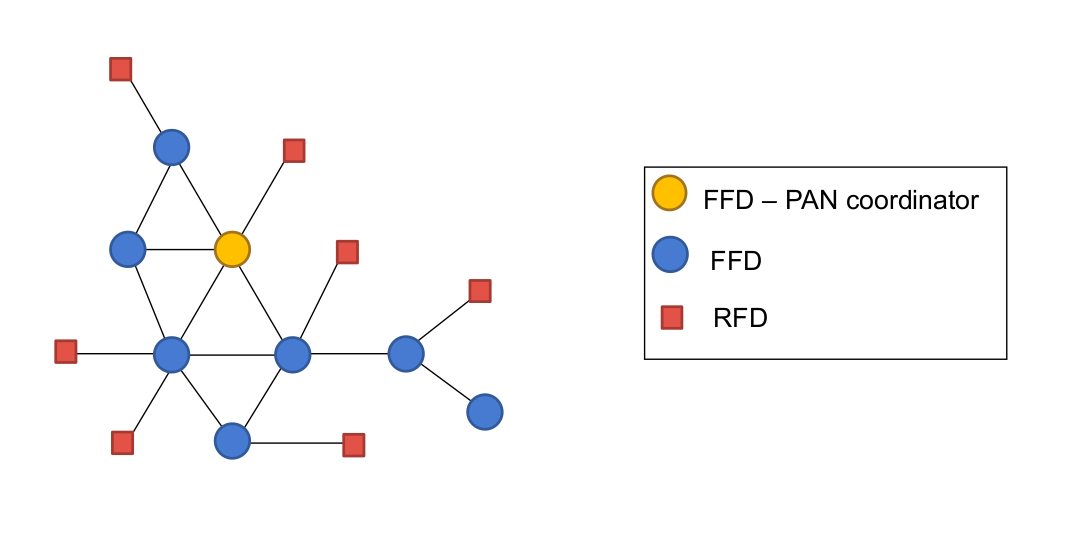
\includegraphics{images/802_p2p.png}
      \label{fig:802_p2p}
   \end{figure}
   % \item \textbf{Cluster-tree}: a coordinator communicates with other coordinators, which in turn communicate with other nodes.
\end{itemize}
   
\section{Channel Access}
There are two options for channel access:
\begin{enumerate}
   \item \textbf{Superframe}:
   used in star and tree-structured p2p networks, enforces the synchronization of devices.
   \item \textbf{Non beacon-enabled} (\textit{Without superframe}):
   this schema is more general and supports communication in arbitrary p2p networks.
\end{enumerate}

\subsection{Superframe}
\begin{figure}[htbp]
   \centering
   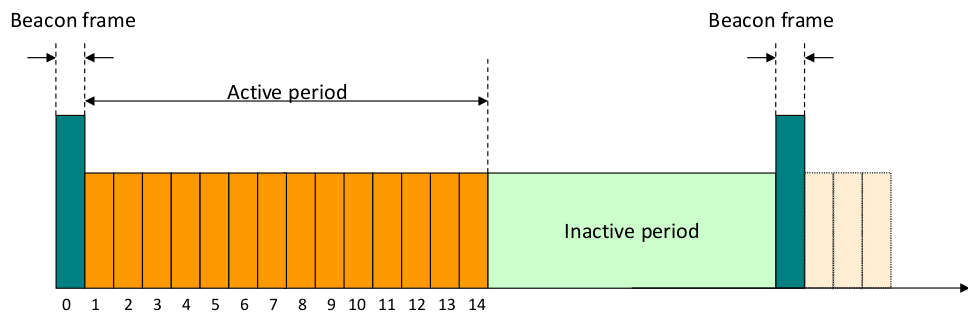
\includegraphics{images/802_superframe_beacon.png}
   \caption{Beacons and superframes in 802.15.4}
   \label{fig:802_superframe_beacon}
\end{figure}

There are equally sized time slots, with the first one being the beacon frame, sent by the PAN coordinator to begin the superframe.

The end devices can communicate with the coordinator in the
remaining time slots.
The beacons are used to:
\begin{itemize}
   \item Identify the PAN,
   \item Synchronize the devices in the PAN,
   \item Communicate the structure of the superframe.
\end{itemize}

The superframe comprises an active and an inactive portion. The active portion is made up of (max) 16 time slots and indicates where the communication has to happen.
It is divided into two parts:
\begin{enumerate}
   \item \textit{Contention Access Period} (\textbf{CAP})
   which comprises up to 15 time slots and the devices here have to ``compete'' to access the channel.
   \begin{itemize}
      \item a device shall wait for a random number of slots first.
      \item if the slot is busy the device shall wait for another random number of slots before
      trying again.
      \item If the channel is idle, the device can transmit
      \item Once the transmission starts, the \ul{node keeps the medium until the end of the frame}
   \end{itemize}
   \item (\ul{optional}) \textit{Contention Free Period} (\textbf{CFP}), which occupies the last time slots of the active period and is meant for low-latency applications or applications with specific data bandwidth.\\
   It is divided into \textit{Guaranteed Time Slots} (\textbf{GTS})
   \begin{itemize}
      \item Each GTS assigned by the PAN coordinator to a specific application.
      \item The application accesses the GTS without contention.
      \item The GTS may comprise more than one time slots.
      \item Up to 7 GTS within a single CFP, and each may last more than one time slot.
   \end{itemize}
   \note{\textit{What if there are too many GTS requests by application?}\\
   The coordinator answers ``picche''  \smiley
   }
\end{enumerate}

\subsection{Non beacon-enabled}
In this scenario \ul{coordinators} (PAN coordinator and routers) \ul{are always on} and ready to receive data from the end-devices, and there are no beacons or slots: communication based on unslotted \texttt{CSMA-CA} protocol.

Data transfer from coordinators to end-devices is
\textbf{poll-based}: the end device periodically wakes up and polls the coordinator for pending messages, and then the coordinator either sends back the pending messages or signals that no message is pending.

\note{Clearly this is possible because the coordinators are expected to be always on.}

\subsection{Trasferring data}
Data transfer may be of three types, and have different implementations for beacon and non-beacon enabled networks:
\begin{enumerate}
   \item \textit{End-device to coordinator (or router)}
   \item \textit{Coordinator (or router) to end-device}
   \item \textit{Peer to peer.}
\end{enumerate}

\newpage
\subsubsection{Beacon enabled}

\begin{enumerate}
   \item \textit{Data transfer from an end device $\longrightarrow$ coordinator}:
   \begin{paracol}{2}
      \begin{figure}[htbp]
         \centering
         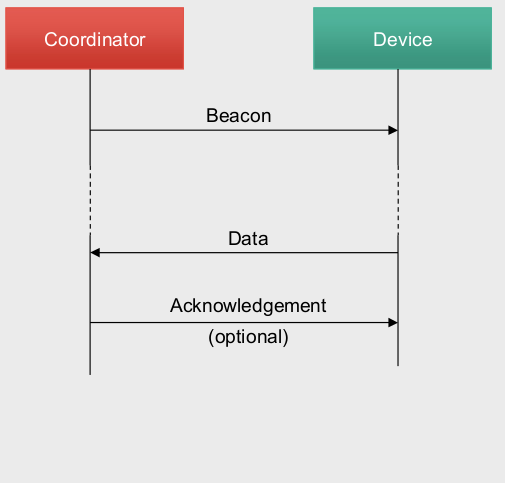
\includegraphics[width=0.6\columnwidth]{images/802_datatransfer_1.png}
         \label{fig:802_datatransfer_1}
      \end{figure}
      
      \switchcolumn
      \colfill
      \begin{enumerate}
         \item The end device first waits for the network beacon to synchronize with the superframe.
         \item If it owns a GTS it uses it without contention, otherwise it transmits the data frame to the coordinator using the slotted CSMA-CA protocol in one of the frames in the CAP period
         \item The coordinator may optionally send an acknowledgement
      \end{enumerate}
      \colfill

   \end{paracol}
      \item \textit{Data transfer from a coordinator $\longrightarrow$ end device}:
   \begin{paracol}{2}
      \colfill
      \begin{figure}[htbp]
         \centering
         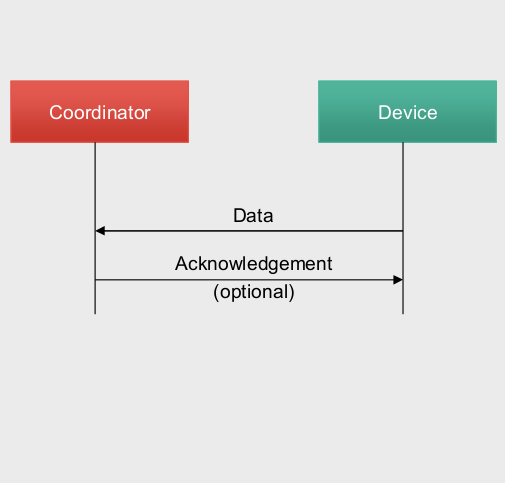
\includegraphics[width=0.6\columnwidth]{images/802_datatransfer_2.png}
         \label{fig:802_datatransfer_2}
      \end{figure}
      \colfill
      \switchcolumn
      
      \begin{enumerate}
      \item The coordinator stores the message and signals that the message is pending in the beacon;
      \item The end-device sleeps most of the time and it occasionally listens to the beacon to check for pending messages, and it notices that there is one, it requests the message to the coordinator.
      \item The coordinator sends the pending message in a
      successive slot of the CAP
      \item The device sends a \textit{mandatory} acknowledgment frame in a successive time slot, so that the coordinator may remove the pending message from its list
   \end{enumerate}
\end{paracol}
   \item \textit{Data transfer in Peer to peer}:
   \begin{itemize}
      \item Between the coordinator (or a router) and an end-device one of the previous schemes is used.
      But this is not possible between two end-devices, because they cannot communicate directly.
      \item Between the coordinator and a router (or between two routers), the sender must first synchronize with the destination beacon and
      act as an end device.
      \note{The measures to be taken in order to synchronize coordinators are beyond the scope of the IEEE 802.15.4 standard. \smiley}
   \end{itemize}
\end{enumerate}

\newpage
\subsubsection{Non beacon-enabled}
\begin{enumerate}
   \item \textit{Data transfer from an end device $\longrightarrow$ coordinator:}
   \begin{paracol}{2}
      \colfill
      
      \begin{figure}[htbp]
         \centering
         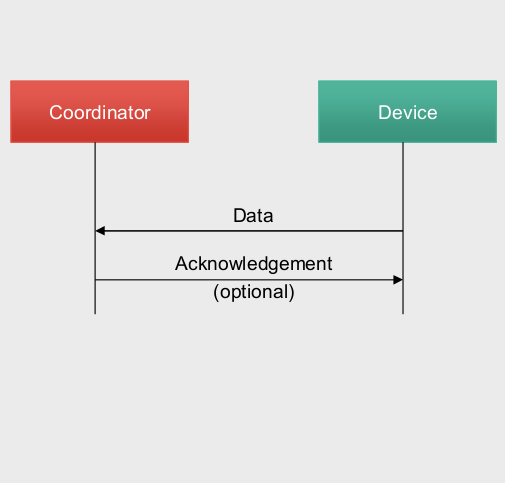
\includegraphics[width=0.6\columnwidth]{images/802_datatransfer_3.png}
         \label{fig:802_datatransfer_3}
      \end{figure}
      \colfill
      \switchcolumn
      \colfill
      \begin{itemize}
         \item the end device simply transmits its data frame to the coordinator using unslotted CSMA-CA, assuming that the coordinator is always on.
         \item The coordinator acknowledges the successful reception of the data by transmitting an \textit{optional} acknowledgment frame
      \end{itemize}
      \colfill
   \end{paracol}
   \item \textit{Data transfer from a coordinator $\longrightarrow$ end device}:
   \begin{paracol}{2}
      \colfill
      
      \begin{figure}[htbp]
         \centering
         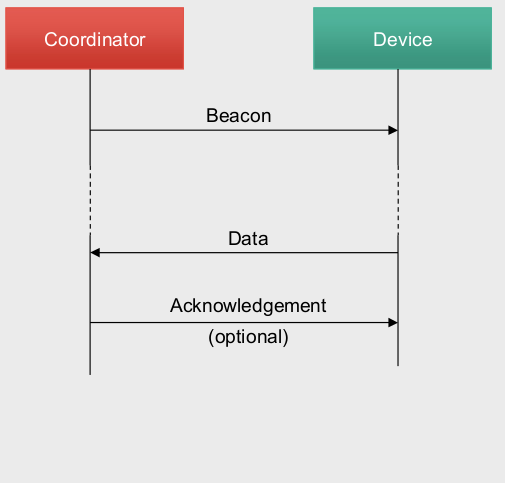
\includegraphics[width=0.6\columnwidth]{images/802_datatransfer_4.png}
         \label{fig:802_datatransfer_4}
      \end{figure}
      \colfill
      \switchcolumn
      \colfill
      \begin{enumerate}
         \item The coordinator stores the message and waits for
         the device to request for the data.
         \item A device can poll the coordinator for pending messages by transmitting a Data request (using unslotted CSMA-CA).
         \item The coordinator send an ack for the request.
         \item The coordinator transmits the pending message(s) to the devices.
         \note{If none present, an empty message is sent}
         \item The device sends an ack and the coordinator discards the sent messages. 
      \end{enumerate}
      \colfill
   \end{paracol}
   \item \textit{Data transfer in Peer to peer}:
   \begin{enumerate}
      \item Each device may communicate with every other device in its radio range
      \item The devices will need to remain always active or to synchronize with each other.
      {\ns\note{Bad!}}
      \begin{itemize}
         \item In the first case the device can directly transmit the data.
         \item In the latter case the \ul{devices synchronization is beyond the scope of the IEEE 802.15.4 standard} (it is left to the upper layers.)
      \end{itemize}
   \end{enumerate}
\end{enumerate}

\section{Services - MAC Layer}

The MAC layer provides \textbf{Data services} by exploiting only three primitives
\begin{enumerate} 
   \item \texttt{DATA.request}: invoked by the upper layer to send a message to another device  
   \item \texttt{DATA.confirm}: reports the result of a transmission requested with a previous \texttt{DATA.request} primitive to the upper layer 
   \item \texttt{DATA.indication}: corresponds to a receive primitive: it is generated by the MAC layer on receipt of a message from the physical layer to pass the received message to the upper layer
\end{enumerate} request, confirm and indication primitives.
\nl

The MAC layer also provides \textbf{Management services}:
\begin{itemize}
   \item PAN initialization
   \item Detection of existing PANs
   \item Devices association/disassociation
   \item Other service
\end{itemize}


\subsection{Associating}
Considering the \textbf{Associate Protocol} from the end-device perspective:
it is invoked by a device willing to associate with a PAN that has already been identified by a preliminary execution of the SCAN service; this procedure thus applies to beacon-enabled networks.\\
The protocol is fairly simple:

\begin{figure}[htbp]
   \centering
   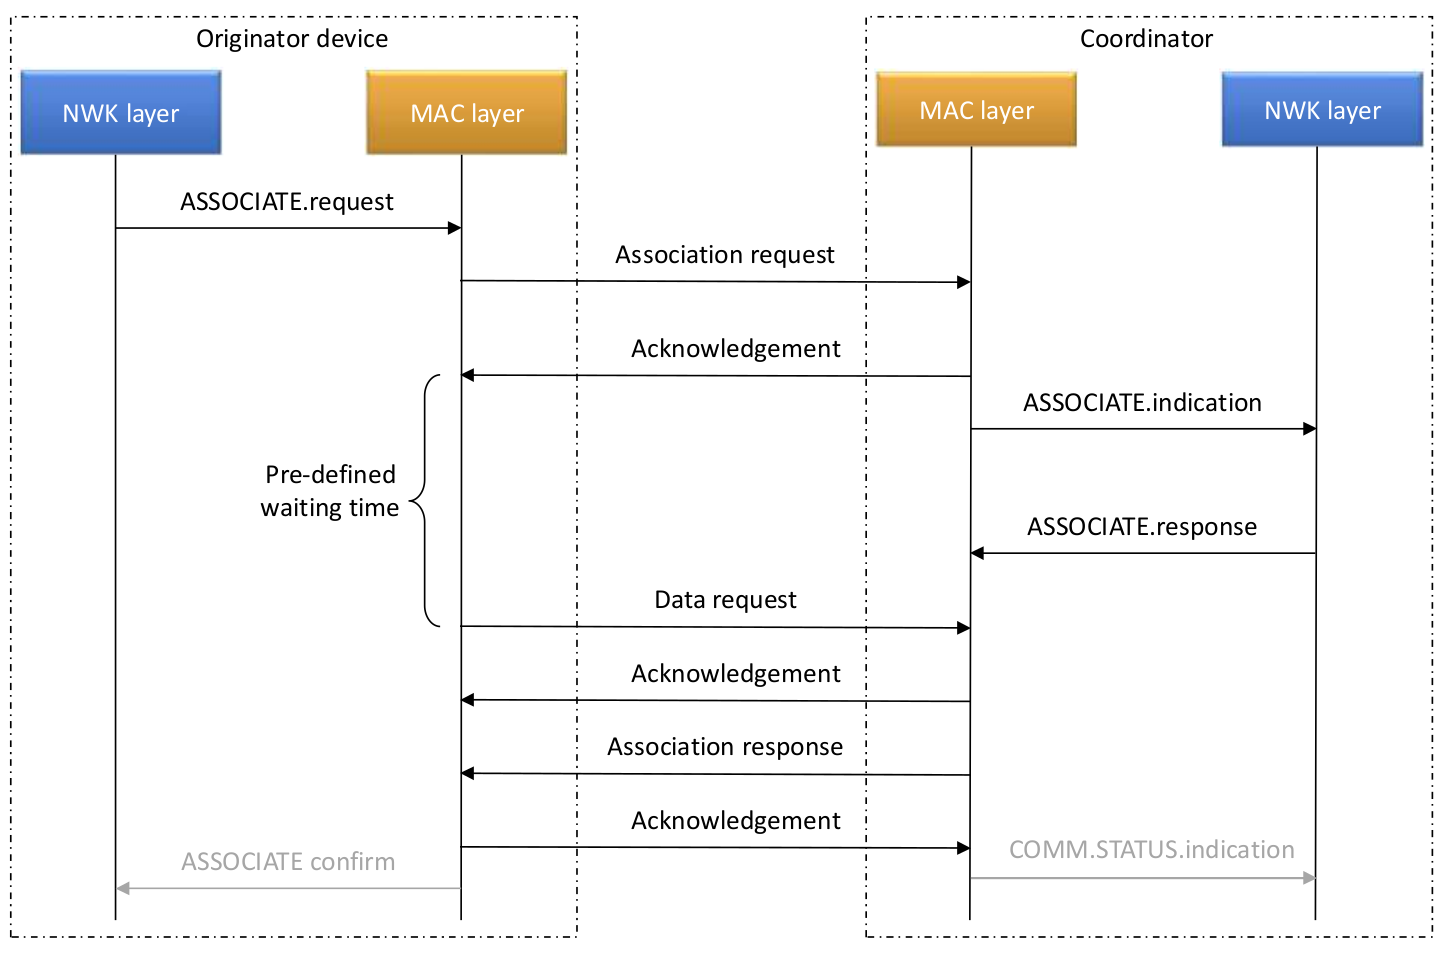
\includegraphics{images/802_associate.png}
   \caption{Associate protocol in 802.15.4}
   \label{fig:802_associate}
\end{figure}

\begin{paracol}{2}
   \begin{enumerate}
      \item The ASSOCIATE.request primitive is sent by the device and has as parameters:
      \begin{enumerate}
         \item the PAN identifier
         \item the coordinator address
         \item the 64-bits extended IEEE address of the device
      \end{enumerate}
      Such request message is sent during the CAP using the slotted CSMA-CA protocol.\\
      Since the device has not yet joined the network, it uses its MAC to send the message.
      \item The coordinator answers with an \texttt{ACK}, which however doesn't mean that the device has joined the network.
      \item The coordinator forwards the association request to the network layer, which in case of acceptance sends an \texttt{ASSOCIATE.response} primitive to the MAC layer, indicating both the MAC of the end-device and its ``associated'' \textit{16-bits address}.
      \item After some predefined time, the end device requests the address, followed by an exchange of ACKs
      \item Lastly the end-device MAC layer sends an \texttt{ASSOCIATE.confirm} primitive to the upper layer.
   \end{enumerate}
   
   \switchcolumn
   
   \begin{figure}[htbp]
      \centering
      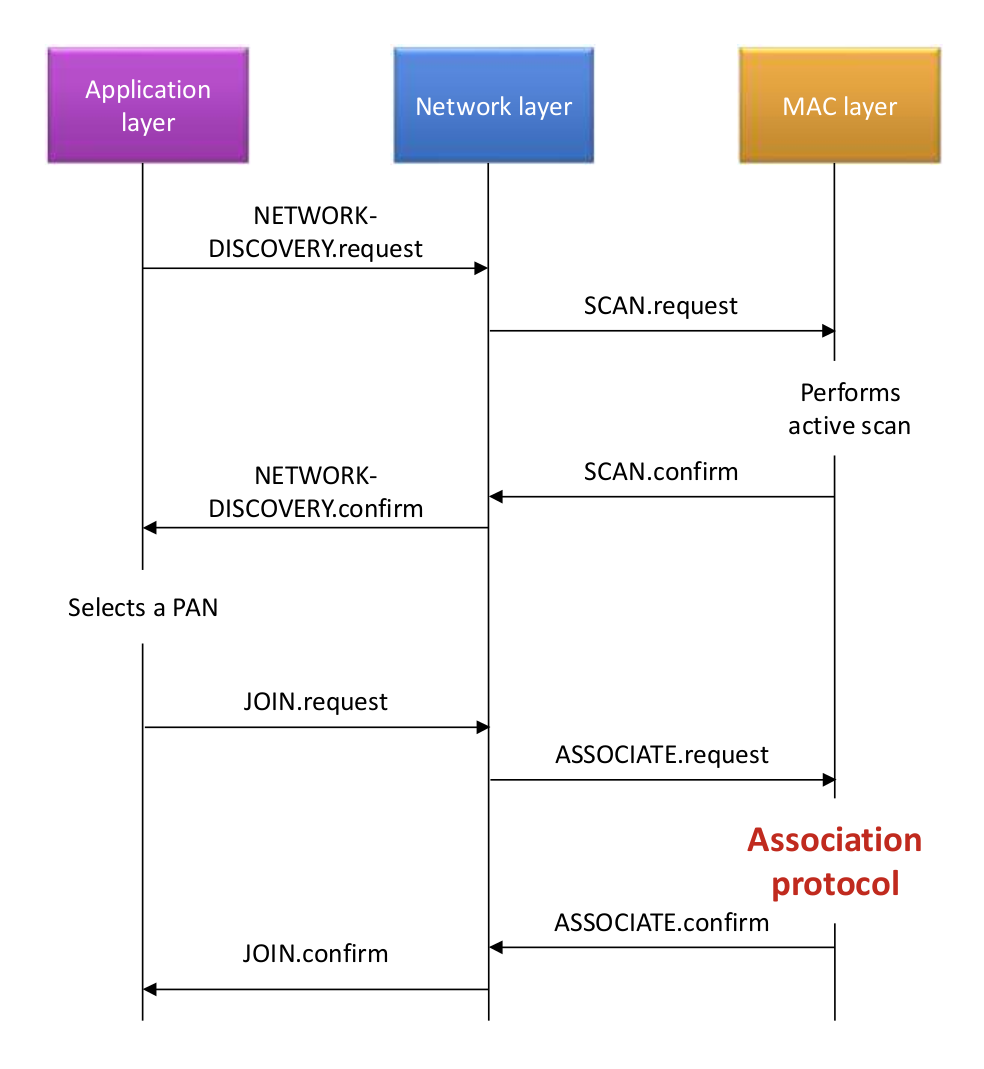
\includegraphics{images/802_join.png}
      \caption{The associate protocol takes place in the last part of the ZigBee network join process}
      \label{fig:802_join}
   \end{figure}
   
\end{paracol}

\framedt{Security services}{
   The MAC layer provides some security features:
   \begin{itemize}
      \item Access control through ACLs
      \item Symmetric Data encryption using keys provided by upper layers
      \item Frame integrity using the same keys of encryption
      \item Sequential freshness of frames
   \end{itemize}
}